%!TEX root = ../dokumentation.tex

%TODO: Einleitung überarbeiten
\chapter{Setup}\label{cha:Setup}
Lorem ipsum \ac{OS} Ubuntu  dolor sit amet, consetetur sadipscing elitr, sed diam nonumy eirmod tempor invidunt ut labore et dolore magna aliquyam erat, sed diam voluptua. At vero eos et accusam et justo duo dolores et ea rebum. Stet clita kasd gubergren, no sea takimata sanctus est Lorem ipsum dolor sit amet. Lorem ipsum dolor sit amet, consetetur sadipscing elitr, sed diam nonumy eirmod tempor invidunt ut labore et dolore magna aliquyam erat, sed diam voluptua. At vero eos et accusam et justo duo dolores et ea rebum. Stet clita kasd gubergren, no sea takimata sanctus est Lorem ipsum dolor sit amet. Lorem ipsum dolor sit amet, consetetur sadipscing elitr, sed diam nonumy eirmod tempor invidunt ut labore et dolore magna aliquyam erat, sed diam voluptua. At vero eos et accusam et justo duo dolores et ea rebum. Stet clita kasd gubergren, no sea takimata sanctus est Lorem ipsum dolor sit amet. 

Duis autem vel eum iriure dolor in hendrerit in vulputate velit esse molestie consequat, vel illum dolore eu feugiat nulla facilisis at vero eros et accumsan et iusto odio dignissim qui blandit praesent luptatum zzril delenit augue duis dolore te feugait nulla facilisi. Lorem ipsum dolor sit amet, consectetuer adipiscing elit, sed diam nonummy nibh euismod tincidunt ut laoreet dolore magna aliquam erat volutpat. 

Ut wisi enim ad minim veniam, quis nostrud exerci tation ullamcorper suscipit lobortis nisl ut aliquip ex ea commodo consequat. Duis autem vel eum iriure dolor in hendrerit in vulputate velit esse molestie consequat, vel illum dolore eu feugiat nulla facilisis at vero eros et accumsan et iusto odio dignissim qui blandit praesent luptatum zzril delenit augue duis dolore te feugait nulla facilisi. 

\newpage
\begin{lstlisting}[language=bash, caption={Konfiguration des Hadoop Users}, label=lis:KonfHadoopUser]
# Create usergroup and user
sudo addgroup hadoop
sudo adduser -ingroup hadoop hduser

# login as hadoop user and create rsa key
su - hduser
ssh-keygen -t rsa -P ""

# add to authorized keys
cat $HOME/.ssh/id_rsa.pub >> $HOME/.ssh/authorized_keys

# Initial login on host via ssh
ssh localhost
\end{lstlisting}

\begin{lstlisting}[language=bash, caption={Herunterladen und entpacke von Hadoop}, label=lis:HerunterladenUndEntpacken]
$ cd /usr/local
$ sudo wget http://apache.openmirror.de/hadoop/common/current
            /hadoop-2.7.1.tar.gz
$ sudo tar xfz hadoop-2.7.1.tar.gz
$ sudo mv hadoop-2.7.1 hadoop
$ sudo chown -R hduser:hadoop hadoop
\end{lstlisting}

\newpage
\begin{lstlisting}[language=bash, caption={Umgebungsvariablen für Hadoop}, label=lis:Umgebungsvariablen]
# Java
export JAVA_HOME=/usr/lib/jvm/java-7-openjdk-amd64

# Hadoop
export HADOOP_INSTALL=/usr/local/hadoop
export PATH=$PATH:$HADOOP_INSTALL/bin
export PATH=$PATH:$HADOOP_INSTALL/sbin
export HADOOP_MAPRED_HOME=HADOOP_INSTALL
export HADOOP_COMMON_HOME=HADOOP_INSTALL
export HADOOP_HDFS_HOME=HADOOP_INSTALL
export HADOOP_YARN_HOME=HADOOP_INSTALL
\end{lstlisting}

\begin{figure}[h]
	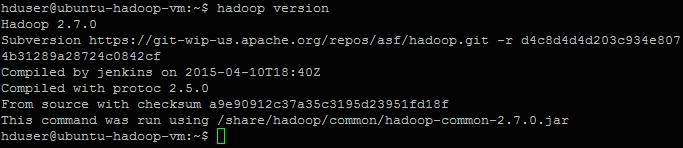
\includegraphics[width=1\textwidth]{hadoop_version.png}
	\caption{Ergebnis für die Kommandozeileneingabe \textit{hadoop version}}
	\label{fig:ErgebnisKomandozeileneingabe}
\end{figure}

\pagebreak
\begin{lstlisting}[language=XML, caption=Konfiguration in der core-site.xml, label=lis:KonfCoreSite]
<configuration>
	<property>
		<name>fs.defaultFS</name>
		<value>hdfs://localhost:9000</value>
	</property>
</configuration>
\end{lstlisting}